\documentclass[../../main]{subfiles}

\renewcommand\thesection{\arabic{section}}


\begin{document}

\section{ESP32} \label{sec:}

\begin{center}
    {\begin{minipage} [c] {0.55\textwidth}
        \esp is a well \emph{documented} and a \emph{powerful} \emph{micro-controller} available in
        the market. The \emph{Espressif} makes a wide verity
        of micro-controllers, the one we have chosen is the \esp. And \esp comes in different \emph{dev
        boards}. From those we will be using the board \texttt{ESP32-D0WD-V3}.

        Please refer figure \ref{fig:esp32DevBoard} and \ref{fig:esp32PinDiagram} for a quick glance
        at the device.
    \end{minipage}
    \hfill
    \begin{minipage} [c] {0.35\textwidth}
        \centering
        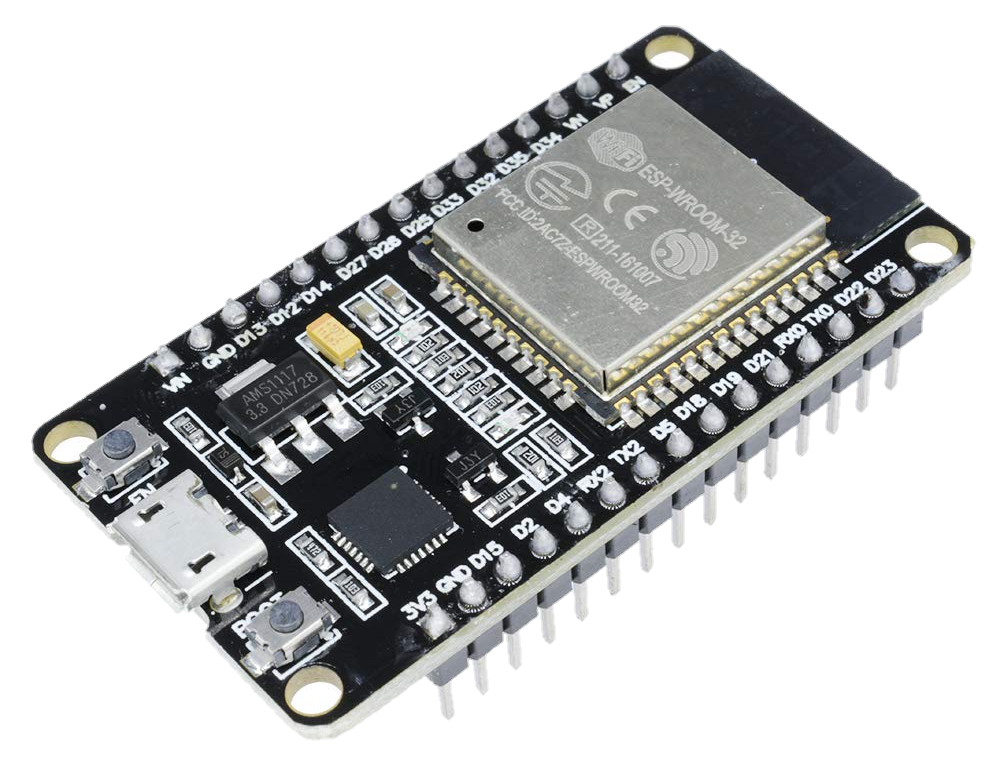
\includegraphics [
            max width = \IGXMaxWidth,
            max height = \IGXMaxHeight,
            \IGXDefaultOptionalArgs,
        ] {pics/esp32.png}
        \captionof{figure} {
            \texttt{ESP32-D0WD-V3} board.
            \label{fig:esp32DevBoard}
        }
    \end{minipage}\hfill}
\end{center}


Even though the \texttt{ESP32-D0WD-V3} module has a lot of pins, freely usable
pins are limited. There are \emph{strapping} pins that are needed to be floating
while booting. And pins that are used for \emph{flash} memory. Another thing
to note is that, not every pins of \esp can be used as output pins, as they lack
internal pull ups or pull downs.

\begin{center}
    {\begin{minipage}[c] {0.35\textwidth}
        \centering

        \includegraphics [
            max width = \IGXMaxWidth,
            max height = \IGXMaxHeight,
            \IGXDefaultOptionalArgs,
        ] {tikzpics/endAbsESPPinout.pdf}
        \captionof{figure} {
            Pin diagram of \texttt{ESP32-D0WD-V3} Board.
            \label{fig:esp32PinDiagram}
        }

    \end{minipage}
    \hfill
    \begin{minipage}[c] {0.52\textwidth}
        \esp has $2$ ADCs,
        each of these has multiple channels. But there is a caveat, the ADC $2$ cannot
        be used while using the WiFi is being used. So we need to use ADC $1$ for our
        voltage measurements. And we need to choose\footnote{as multiplexer read pin, see
        section \ref{sec:multiplexerSystem}, for more information.} a pin that can:

        \begin{itemize}
            \item Use ADC $1$.
            \item Be configured as input.
            \item Be configured as output.
        \end{itemize}

        Luckily \texttt{GPIO\_32} can be used like this, which is the \texttt{D32} pin that
        can be seen in figure \ref{fig:esp32PinDiagram}.

    \end{minipage}}

\end{center}

\alertNote{
    \emph{Strapping} pins can be used as \emph{GPIO}, but we just need to make sure that they are
    \emph{floating} during the boot up process of \esp.
}

Another highlight is \esp features a dual core Xtensa\footnote{processor architecture.} processor. And runs a
modified\footnote{FreeRTOS is meant for single core processors.} version of \emph{FreeRTOS},
which enables SMP\footnote{Symmetric Multi-Processing}. That means, with \emph{Espressif}'s
\texttt{esp-idf}\footnote{Integrated Development Framework.} we can have all the goodness
of a fully featured Real Time OS. And WiFi capabilities ensures the seamless connection, as
it supports different WiFi modes, including \emph{station mode}, \emph{access point mode},
\emph{combined mode}\footnote{can be used as \emph{station} and as an \emph{access point} simultaneously.}, etc.

\alertNote{
    Right now, we will be using \esp entirely in \emph{wifi station mode}.
}

\begin{center}
    {\begin{minipage}[c] {0.42\textwidth}
        \centering

        \includegraphics [
            max width = \IGXMaxWidth,
            max height = \IGXMaxHeight,
            \IGXDefaultOptionalArgs,
        ] {../../tikzpics/endAbsESP.pdf}
        \captionof{figure} {
            A simplified diagram of \texttt{ESP32-D0WD-V3} Board.
            \label{fig:esp32SimpleDiagram}
        }

    \end{minipage}
    \hfill
    \begin{minipage}[c] {0.52\textwidth}
        Following chapters will go through the pin allocation, as we design each of the systems of the
        incubator. Also, take a look at the simplified version of \texttt{ESP32-D0WD-V3} Board in figure
        \ref{fig:esp32SimpleDiagram}, that will be used in the following chapters for the sake of
        simplicity.
    \end{minipage}}

\end{center}


\end{document}
